\apendice{Documentación}\label{documentacion}

\section{Introducción}
El siguiente apéndice se compone de tres apartados principales: El primero presenta la estructura de directorios en la que se organiza el proyecto; el segundo apartado documenta cómo descargar los datos empleados para entrenar y evaluar los modelos, así como las instrucciones para instalar los componentes \textit{software} requeridos por los programas desarrollados en este trabajo; por último, en el tercer apartado, se especifican los comandos necesarios para ejecutar los \textit{scripts} disponibles.

\section{Estructura de directorios}

A continuación se encuentra la estructura de directorios y ficheros de este Trabajo Fin de Máster. Esta estructura se divide en dos directorios principales: \textit{data/}, que contiene el \textit{dataset} de KITTI; y DPT/, que es un \textit{fork} del repositorio de la publicación original \cite{visiontransformersDPT} disponible en \url{TODO}.

En este segundo directorio, se encuentran a su vez los subdirectorios: 

\textit{dpt/}, que agrupa los \textit{scripts} que definen la arquitectura, modificados para incluir los distintos cambios presentados en este trabajo; \textit{input/} y \textit{output{\_}monodepth/} contienen respectivamente, las entradas de los \textit{scripts} de inferencia y sus salidas; \textit{util/} incluye archivos con funciones de utilidad general; \textit{wandb{\_}sweeps/} agrupa los distintos ficheros YAML que definen las búsquedas de hiperparámetros que se han llevado a cabo empleando wandb; por último, en \textit{weights/} se encuentran los ficheros con los parámetros entrenados de los distintos modelos.

En cuanto a los ficheros situados de \textit{DPT/}: 

\texttt{KITTIDataset.py}, define el \texttt{torch.utils.data.Dataset} adaptado para cargar las imágenes y anotaciones de KITTI; \texttt{attention{\_}complexity.py} y \texttt{inference{\_}speed.py} ejecutan, respectivamente, distintas capas y distintos modelos para obtener métricas sobre su velocidad, tamaño, y número de operaciones; \texttt{eval{\_}with{\_}pngs.py} y \texttt{run{\_}eval{\_}with{\_}pngs{\_}.sh} calculan métricas del rendimiento de los modelos; \texttt{run{\_}monodepth.py} lleva a cabo la inferencia de profundidad; y por último, \texttt{train.py} y \texttt{train{\_}utils.py} gestionan el entrenamiento de modelos.

\pagebreak

\dirtree{%
.1 TFM/.
.2 data/.
.3 KITTI/.
.4 data{\_}depth{\_}annotated/.
.5 train/.
.6 YYYY{\_}MM{\_}DD{\_}drive{\_}XXXX{\_}sync/.
.5 val/.
.6 YYYY{\_}MM{\_}DD{\_}drive{\_}XXXX{\_}sync/.
.4 raw/.
.5 YYYY{\_}MM{\_}DD/.
.4 train{\_}files{\_}eigen{\_}full{\_}fix.txt.
.4 val{\_}files{\_}eigen{\_}full{\_}fix.txt.
.2 DPT/.
.3 dpt/.
.4 ConvEmbeddingWrapper.py.
.4 base{\_}model.py.
.4 blocks.py.
.4 models.py.
.4 transforms.py.
.4 vit.py.
.3 input/.
.3 output{\_}monodepth/.
.3 util/.
.4 io,py.
.4 misc.py.
.3 wandb{\_}sweeps/.
.4 *.yml.
.3 weights/.
.4 *.pt.
.3 KITTIDataset.py.
.3 README.md.
.3 attention{\_}complexity.py.
.3 eval{\_}with{\_}pngs.py.
.3 inference{\_}speed.py.
.3 requirements.txt.
.3 run{\_}eval{\_}with{\_}pngs.sh.
.3 run{\_}monodepth.py.
.3 train.py.
.3 train{\_}utils.py.
}

\section{Descarga de datos e instalación de \textit{software}}
A continuación se encuentran los pasos necesarios para descargar los datos empleados durante el proyecto e instalar el \textit{software} de los entornos de desarrollo. \textbf{Parte de estas instrucciones son específicas para equipos con sistema operativo Ubuntu 20.04 LTS}, por lo que se proporcionan enlaces con información relevante para otras distribuciones. Además, se presupone que el equipo en el que se va a llevar a cabo el proceso de instalación tiene una tarjeta gráfica NVIDIA con los controladores gráficos (\textit{drivers}) correspondientes correctamente instalados.

\subsection{Descarga de datos}
El \textit{dataset} empleado para entrenar y evaluar los distintos modelos es el conjunto de datos de KITTI para estimación de profundidad en imágenes monoculares. Este \textit{dataset} se puede descargar a través de su página web, tanto los datos en bruto (\textit{synced+rectified data}) \url{http://www.cvlibs.net/datasets/kitti/raw_data.php}, como las anotaciones (\textit{annotated depth maps}) \url{http://www.cvlibs.net/datasets/kitti/eval_depth.php?benchmark=depth_prediction}. 

Los ficheros que definen las conjuntos de entrenamiento y de evaluación se encuentran disponibles en el siguiente repositorio \url{https://github.com/nianticlabs/monodepth2/tree/master/splits/eigen_full}. 

Por último, las imágenes del conjunto de \textit{test} (\textit{kitti{\_}eval{\_}dataset.zip}), se han descargado agrupadas desde \url{https://github.com/isl-org/DPT/blob/main/EVALUATION.md}.

\subsection{Docker Engine}
Para utilizar los contenedores de Docker, es necesario instalar el Docker Engine. Estas instrucciones son para sistemas con Ubuntu. En el siguiente enlace (\url{https://docs.docker.com/engine/install/}), hay disponibles instrucciones para otras distribuciones.

\begin{enumerate}
\item Eliminamos versiones anteriores de Docker (en caso de existir):

\texttt{\$ sudo apt-get remove docker docker-engine docker.io containerd runc}

\item Instalamos paquetes necesarios para usar un repositorio a través de HTTPS:

\texttt{\$ sudo apt-get update}

\texttt{\$ sudo apt-get install apt-transport-https ca-certificates curl \textbackslash \\ gnupg lsb-release}

\item Añadimos la clave GPG de Docker:

\texttt{\$ curl -fsSL https://download.docker.com/linux/ubuntu/gpg | sudo gpg \textbackslash \\ {-}{-}dearmor -o /usr/share/keyrings/docker-archive-keyring.gpg}

\item Configuramos el repositorio de Docker:

\texttt{\$ echo \textbackslash \\ 
"deb [arch=amd64 signed-by=/usr/share/keyrings/docker-archive-keyring.gpg] \textbackslash \\ 
https://download.docker.com/linux/ubuntu \$(lsb{\_}release -cs) stable"{ }| \textbackslash \\ sudo tee /etc/apt/sources.list.d/docker.list >{ }/dev/null}

\item Instalamos Docker:

\texttt{\$ sudo apt-get update}

\texttt{\$ sudo apt-get install docker-ce docker-ce-cli containerd.io}

\item Por último, comprobamos que la instalación se haya llevado a cabo correctamente:

\texttt{\$ sudo docker run hello-world}

% \par\noindent\rule{0.965\textwidth}{0.4pt}

\end{enumerate}

Docker ya está instalado, pero es necesario ejecutarlo como superusuario. Para remediar esto (opcional), es posible crear un grupo \texttt{"docker"} y añadir nuestro usuario. Al hacer esto \textbf{pueden aparecer riesgos de seguridad}. Se puede encontrar más información en:

\begin{itemize}

\item \url{https://docs.docker.com/engine/install/linux-postinstall/}

\item \url{https://docs.docker.com/engine/security/#docker-daemon-attack-surface}

\end{itemize}


\begin{enumerate}

\item Añadimos un grupo \texttt{"docker"}:

\texttt{\$ sudo groupadd docker}

\item Añadimos nuestro usuario al grupo creado:

\texttt{\$ sudo usermod -aG docker \$USER}

\item Salimos y volvemos a iniciar la sesión para re-evaluar la pertenencia a grupos. En sistemas Linux también se puede ejecutar \texttt{newgrp docker}. 

\item Ahora es posible ejecutar el contenedor \texttt{hello-world} sin usar \texttt{sudo}.

\texttt{\$ docker run hello-world}

% \texttt{\$ sudo chown "\$USER":"\$USER"{}{ }/home/"\$USER"{}/.docker -R}
% \texttt{\$ sudo chmod g+rwx "\$HOME/.docker"{} -R}

\end{enumerate}

Por otro lado, es posible configurar el servicio de Docker para que se inicie automáticamente al encender el sistema a través de \texttt{systemctl}:

\begin{itemize}

\item \texttt{\$ sudo systemctl enable docker.service}

\item \texttt{\$ sudo systemctl enable containerd.service}

\end{itemize}

\subsection{NVIDIA Container Toolkit}
Una vez instalado el Docker Engine, es necesario instalar el NVIDIA Container Toolkit, que envuelve la instalación anterior y traslada las primitivas de CUDA desde el CUDA instalado dentro de los contenedores al driver de la GPU en el equipo donde se está ejecutando el contenedor. Estas instrucciones son para equipos con distribuciones Ubuntu y Debian. Para los pasos correspondientes en otras distribuciones, consultar la siguiente url: \url{https://docs.nvidia.com/datacenter/cloud-native/container-toolkit/install-guide.html#getting-started}

\begin{enumerate}
\item Configuramos el repositorio y copiamos la clave GPG:

\texttt{\$ distribution=\$(. /etc/os-release;echo \$ID\$VERSION{\_}ID) \textbackslash \\ \&\& curl -s -L https://nvidia.github.io/nvidia-docker/gpgkey | \textbackslash \\ sudo apt-key add - \textbackslash \\ \&\& curl -s -L \textbackslash \\ https://nvidia.github.io/nvidia-docker/\$distribution/nvidia-docker.list | \textbackslash \\ sudo tee /etc/apt/sources.list.d/nvidia-docker.list}

\item Instalamos el paquete correspondiente:

\texttt{\$ sudo apt-get update}

\texttt{\$ sudo apt-get install -y nvidia-docker2}

\item Para terminar la instalación, reiniciamos el servicio de Docker:

\texttt{\$ sudo systemctl restart docker}

\item Para comprobar que la instalación es correcta, podemos ejecutar un contenedor de una imagen con CUDA instalado:

\texttt{\$ docker run {-}{-}rm {-}{-}gpus all nvidia/cuda:11.0-base nvidia-smi}

\end{enumerate}

\begin{figure}[H]
\centering
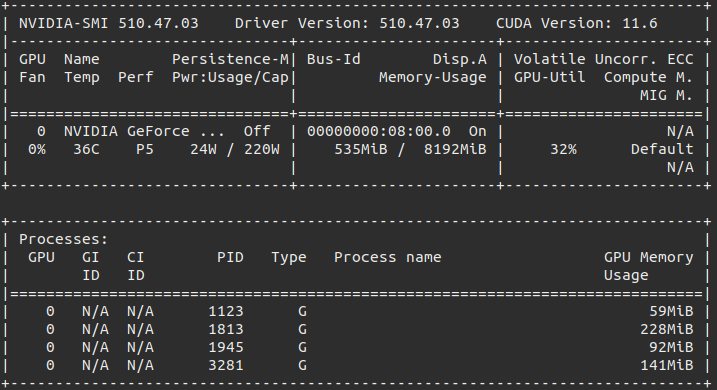
\includegraphics[width=1\linewidth]{imagenes/nvidia-smi.png} 
\captionsetup{width=1\linewidth}
\caption{Resultado del comando \texttt{nvidia-smi} dentro del contenedor.}
\label{fig:performer}
\end{figure}

A pesar de que el comando se ha ejecutado dentro de una imagen con CUDA 11.0, el resultado muestra CUDA 11.6 ya que accede directamente al \textit{driver} del \textit{host} y muestra la versión más alta de CUDA soportada por el \textit{driver} instalado. Se puede encontrar más información sobre esto en: \url{https://github.com/NVIDIA/nvidia-docker/issues/1237#issuecomment-703524943}.

\subsection{Construcción de la imagen de Docker}

Para construir la imagen de Docker, se emplea el Dockerfile incluido en el repositorio, que parte de una imagen con CUDA 11.1 y PyTorch 1.9.0 e instala el software necesario para ejecutar los \textit{scripts} correctamente. El comando a utilizar (si nos encontramos en la misma carpeta que el Dockerfile) es el siguiente, donde los argumentos USER{\_}ID y GROUP{\_}ID se utilizan para crear un usuario en la imagen que corresponda con el del \textit{host} y evitar problemas de permisos, y \$tag será el nombre que se le dará a la imagen:

\texttt{\$ docker build \textbackslash \\
{-}{-}build{-}arg USER{\_}ID=\$(id {-}u) {-}{-}build{-}arg GROUP{\_}ID=\$(id {-}g) {-}{-}tag \$tag .}

Al ejecutar el comando anterior se genera un \textit{build context} del directorio en el que nos encontramos, así que en caso de hacerlo en una carpeta con datos o archivos que no se van a emplear durante la construcción de la imagen podemos redactar un archivo \texttt{.dockerignore} para no considerarlos.

\subsection{Instalación de wandb (Opcional)}

Para poder gestionar las búsquedas de hiperparámetros desde el \textit{host} sin necesidad de entrar a un contenedor, es recomendable (pero no estrictamente necesario) instalar wandb, bien a través del instalador de paquetes de Python (pip) o creando un entorno de Anaconda, entre otras. Tener este paquete instalado, además, facilita el paso de credenciales a los contenedores de Docker a través del comando \texttt{wandb docker{-}run}

\section{Ejecución}

Para poder ejecutar los \textit{scripts} de este proyecto, es necesario crear un contenedor de la imagen previamente construida. Para esto, empleamos el siguiente comando (desde el directorio TFM):

\texttt{\$ wandb docker{-}run {-}{-}gpus all {-}{-}rm {-}it {-}{-}name \$\{tag\}{\_}container 
{-}{-}ipc=host \textbackslash \\ 
{-}p 8888:8888 {-}v \$(pwd):/workspace {-}v /tmp/.X11{-}unix:/tmp/.X11{-}unix {-}e DISPLAY \$tag}

En este comando, \$tag debe corresponderse con el nombre de la imagen creada anteriormente. El resto de opciones de este comando son: \texttt{{-}{-}gpus all}, para usar en el contenedor todas las GPUs disponibles; \texttt{{-}{-}rm}, para eliminar el contenedor y su sistema de ficheros al cerrarlo; \texttt{{-}it}, para hacerlo interactivo y abrir una sesión al iniciarlo; \texttt{{-}{-}ipc=host} para facilitar la comunicación entre procesos de PyTorch; \texttt{{-}p 8888:8888}, para mapear los puertos correspondientes y poder abrir cuadernos jupyter que se ejecutan dentro del contenedor a través del navegador del \textit{host}; por último, la opción \texttt{{-}v \$(pwd):/workspace} monta el directorio actual (TFM) dentro del contenedor, facilitando así el acceso al \textit{dataset} y al código fuente que se encuentran en el \textit{host}.

Además de las ya mencionadas, hay dos opciones más, \texttt{{-}v /tmp/.X11{-}unix:/tmp/.X11{-}unix {-}e DISPLAY}, empleadas para habilitar la visualización y uso de GUIs (por ejemplo, la función \texttt{imshow} de OpenCV) dentro del contenedor.

Tal y como se ha comentado previamente, si wandb no está instalado en el \textit{host}, se puede sustituir \texttt{wandb docker{-}run} por \texttt{docker run}, siendo entonces necesario configurar las credenciales de wandb una vez iniciado el contenedor. 

Una vez iniciado el contenedor, la ejecución de los \textit{scripts} se puede agrupar en:
\begin{itemize}

\item \textbf{Gestionada por wandb}: Como es el caso de los \textit{scripts} \texttt{attention{\_}complexity.py}, \texttt{inference{\_}speed.py} y \texttt{train.py}. Estos procesos iteran sobre distintas configuraciones de modelos y por lo tanto es necesario lanzarlos a través del gestor de ejecuciones de wandb, que se encarga de distribuir la ejecución de las configuraciones en tantos equipos como dispongamos.

\begin{enumerate}

\item Creamos el \textit{sweep} en el \textit{host} con el archivo YAML correspondiente.

\texttt{\$ wandb sweep <fichero{-}YAML>}

\item Lanzamos agentes asociados a dicho \textit{sweep} en los contenedores disponibles (tanto en local como en \textit{cloud} (desde sus respectivos directorios DPT/).

\texttt{\$ wandb agent <usuario>/<nombre{-}proyecto>/<sweep{-}id>}

\end{enumerate}

\item \textbf{No gestionada por wandb}: Por otro lado, la inferencia y evaluación de un modelo concreto en el conjunto de \textit{test} requiere que se especifique la configuración deseada y el fichero de pesos en el \textit{script} \texttt{run{\_}monodepth.py}. Es posible ejecutar este \textit{script} de dos formas (también desde el directorio DPT/):

\begin{itemize}

\item Directamente, ejecutando \texttt{run{\_}monodepth.py}. Por defecto, infiere la profundidad de las imágenes en la carpeta input/ y almacena el resultado en la carpeta output{\_}monodepth/. $\rightarrow$ \texttt{\$ python run{\_}monodepth.py}

\item A través de \texttt{run{\_}eval{\_}with{\_}pngs.sh}, que elimina los resultados anteriores, infiere con los parámetros adecuados el resultado en el conjunto de \textit{test}, y calcula una serie de métricas con las anotaciones correspondientes utilizando el \textit{script} proporcionado en \cite{bts} (\texttt{eval{\_}with{\_}pngs.py}). $\rightarrow$ \texttt{ \$ ./run{\_}eval{\_}with{\_}pngs.sh}

\end{itemize}

\end{itemize}